% Styles
\tikzstyle{block} = [rectangle, thick, minimum width=2.5cm, minimum height=1.5cm,text centered, text width=3cm, draw=black, fill=white]
\tikzstyle{arrow} = [thick, ->, >=stealth]
\tikzstyle{textOutput} = [black,right]
\tikzstyle{textInput} = [black,left]
\tikzstyle{container} = [gray,dashed]

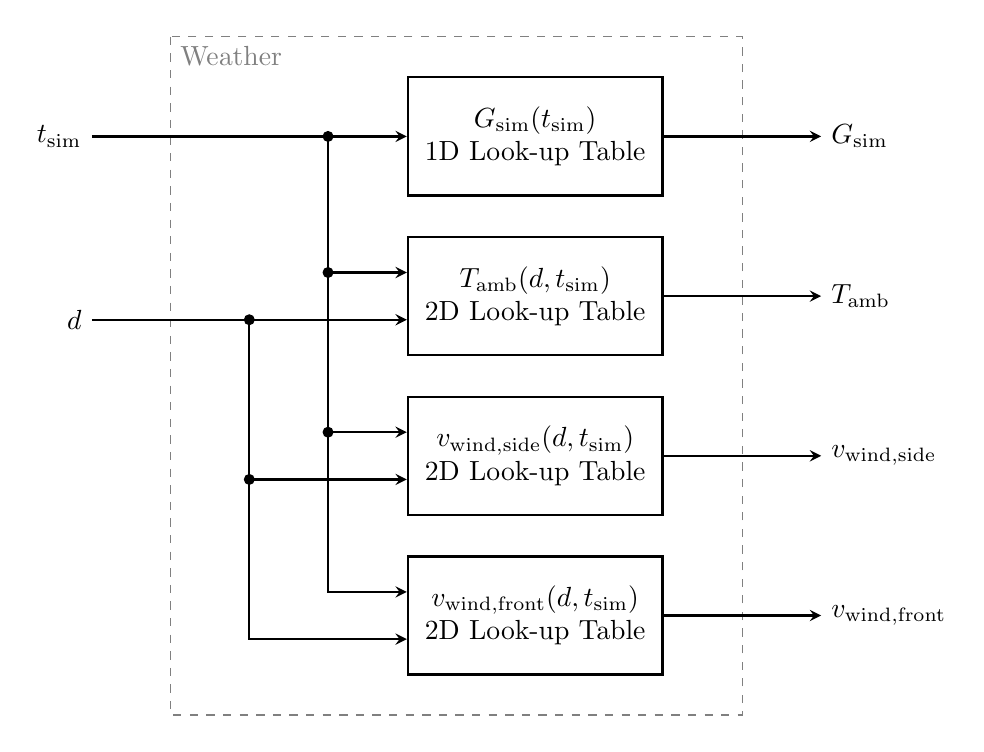
\begin{tikzpicture}
	% Definition
	\def\up{0.3}
	\def\down{-\up}
	\def\radius{0.07}
	
	% Blocks
	\matrix[column sep=1cm, row sep=0.5cm]{
		%first row
		& \coordinate (c12); & & & & & &
		\\
		%second row
		\coordinate (c21); & & & \coordinate (c24); & \node[block] (G) {$G_\mathrm{sim}(t_\mathrm{sim})$ \\ 1D Look-up Table}; & & \coordinate (c27); &
		\\
		%third row
		\coordinate (c31); & & \coordinate (c33); & \coordinate (c34); & \node[block] (T) {$T_\mathrm{amb}(d,t_\mathrm{sim})$ \\ 2D Look-up Table}; & & \coordinate (c37); &
		\\
		%fourth row
		& & \coordinate (c43); & \coordinate (c44); & \node[block] (vs) {$v_\mathrm{wind,side}(d,t_\mathrm{sim})$ \\ 2D Look-up Table}; & & \coordinate (c47); &
		\\
		%fifth row
		& & \coordinate (c53); & \coordinate (c54); & \node[block] (vf) {$v_\mathrm{wind,front}(d,t_\mathrm{sim})$ \\ 2D Look-up Table}; & & \coordinate (c57); &
		\\
		%sixth row
		& & & & & \coordinate (c66); & &
		\\
	};
	
	% Container
	\draw[container] (c12) rectangle (c66);
	\node[gray, anchor=north west] at (c12.north west) {Weather};
	
	% Arrows
	\draw[arrow] (c21) node[textInput] {$t_\mathrm{sim}$} -- (G);
	\draw[arrow] (G) -- (c27) node[textOutput] {$G_\mathrm{sim}$};
	
	\draw[arrow] ([yshift=\down cm]c31) node[textInput] {$d$} -- ([yshift=\down cm]T.west);
	\draw[arrow] (T) -- (c37) node[textOutput] {$T_\mathrm{amb}$};
	\draw[arrow] ([yshift=\up cm]c34) -- ([yshift=\up cm]T.west);
	
	\draw[arrow] (vs) -- (c47) node[textOutput] {$v_\mathrm{wind,side}$};
	\draw[arrow] ([yshift=\up cm]c44) -- ([yshift=\up cm]vs.west);
	\draw[arrow] ([yshift=\down cm]c43) -- ([yshift=\down cm]vs.west);
	
	\draw[arrow] (vf) -- (c57) node[textOutput] {$v_\mathrm{wind,front}$};
	\draw[arrow] ([yshift=\down cm]c33) -- ([yshift=\down cm]c53) -- ([yshift=\down cm]vf.west);
	\draw[arrow] (c24) -- ([yshift=\up cm]c54) -- ([yshift=\up cm]vf.west);
	
	% Dots
	\fill [black] (c24) circle (\radius cm);
	
	\fill [black] ([yshift=\up cm]c34) circle (\radius cm);
	\fill [black] ([yshift=\down cm]c33) circle (\radius cm);
	
	\fill [black] ([yshift=\up cm]c44) circle (\radius cm);
	\fill [black] ([yshift=\down cm]c43) circle (\radius cm);

	
\end{tikzpicture}